\documentclass{article}

\usepackage[version=3]{mhchem} % Package for chemical equation typesetting
\usepackage{siunitx} % Provides the \SI{}{} and \si{} command for typesetting SI units
\usepackage{graphicx} % Required for the inclusion of images
\usepackage{natbib} % Required to change bibliography style to APA
\usepackage{amsmath} % Required for some math elements 
\usepackage{subfigure}
\usepackage[utf8x]{inputenc}
\usepackage[english,russian]{babel}
\usepackage{cmap}
\usepackage{enumitem}
\usepackage{amssymb}

\usepackage{geometry} % Меняем поля страницы
\geometry{left=2cm}% левое поле
\geometry{right=1.5cm}% правое поле
\geometry{top=1cm}% верхнее поле
\geometry{bottom=2cm}% нижнее поле

\usepackage{xcolor}
\usepackage{hyperref}

\usepackage{listings}
\lstset{language=R, basicstyle=\small, extendedchars=\true, breaklines=true, breakatwhitespace=true} 
 
 % Цвета для гиперссылок
\definecolor{linkcolor}{HTML}{0000FF} % цвет ссылок
\definecolor{urlcolor}{HTML}{0000FF} % цвет гиперссылок

\hypersetup{pdfstartview=FitH,  linkcolor=linkcolor,urlcolor=urlcolor, colorlinks=true}

\setlength\parindent{0pt} % Removes all indentation from paragraphs
\renewcommand{\labelenumii}{\arabic{enumi}.\arabic{enumii}.}


%\usepackage{times} % Uncomment to use the Times New Roman font
%%%
\title{Отчет}
\author{Курносов Д.А. }
\date{15.01.2020}
%%%
\makeatletter
\let\thetitle\@title
\let\theauthor\@author
\let\thedate\@date
\makeatother
%%%
\begin{document}
%%%
\begin{titlepage}
        {\centering
            Санкт-Петербургский политехнический университет Петра Великого\\
            Институт прикладной математики и механики\\
            \textbf{Высшая~школа~прикладной~математики~и~вычислительной~физики}\\
        }
        
        \vfill
        
        {\centering
         \Large
            Отчёт по научно-исследовательской работе\\
            на тему:\\
            \textsl{\textquote{Портирование алгоритма субдифференциального метода на язык программирования Python}}\\
        }
        
        \vfill
        
        Студент группы 3640102/00201 \hspace{0.225cm} \rule{4.6cm}{0.4pt} \hspace{0.225cm} Курносов Д.А.\\
        
        Оценка руководителя: \hspace{0.225cm} \rule{3cm}{0.4pt} \hspace{0.225cm} \rule{3cm}{0.4pt} \hspace{0.225cm} Баженов А.Н.\\
        
        {\raggedleft
            \textquote{\rule{1cm}{0.4pt}} \rule{3cm}{0.4pt} 2021 г.\\
        }
        
        \vfill
        
        {\centering
            Санкт-Петербург\\
            2021 г.\\
        }
    \end{titlepage}
\newpage

\tableofcontents
\newpage


%----------------------------------------------------------------------------------------
%	SECTION 1
%----------------------------------------------------------------------------------------
\section{Постановка задачи}

Основной идеей данной работы было изучение субдифференциального метода Ньютона с целью реализации его на языке программирования Python. Была изучена соответствующая литература, а так же алгоритмы, представленные на других языках программирования. 

%----------------------------------------------------------------------------------------
%	SECTION 1
%----------------------------------------------------------------------------------------
\section{Теория}

\subsection{Субдифференциальный метод Ньютона}

Решение интервальных уравнений может быть сведено к решению индуцированных уравнений вида:

\begin{equation}
 \begin{cases}
 \mathcal{F}(y) = 0, \\
 \mathcal{F}(y) = sti(Csti^{-1}(y) \ominus sti^{-1}(y) + d) = sti(Csti^{-1}(y)) - y + sti(d)
 \end{cases}
\end{equation}

\begin{equation}
 \begin{cases}
 \mathcal{G}(y) = 0, \\
 \mathcal{G}(y) = sti(Csti^{-1}(y) \ominus d) = sti(Csti^{-1}(y)) - sti(d)
 \end{cases}
\end{equation}

при помощи погружения $sti:\mathbb{KR}^n \to \mathbb{R}^{2n}$, действующего по правилу:

\begin{equation}
(x_1, x_2, ... , x_n) \mapsto (-\underline{x_1}, -\underline{x_2}, ... , -\underline{x_n}, \ 
                              \bar{x_1}, \bar{x_2}, ... , \bar{x_n}) 
\end{equation}

Иначе говоря, необходимо составить вектор, первые $n$ элементов которого представляют левые концы интервалов, взятые с противоположным знаком, а последующие $n$ компонент - правые концы интервалов.

Одним из инструментов решения уравнения такого вида является субдифференциальный метод Ньютона. Идея данного алгоритма следующая:

\begin{itemize}
  \item Выбирается некоторое приближение $x^{(0)} \in \mathbb{R}^{2n}$
  \item Вычисляется субградиент $D^{(0)}$ отображения $\mathcal{F}$ в данной точке
  \item Полагаем $x^{1} \leftarrow x^{0} - \tau(D^{(k-1)})^{-1}\mathcal{F}(x^{(k-1)})$, \\
  где $\tau \in [0,1]$
\end{itemize}

Условием остановки алгоритма является условие:
\begin{equation}
 \|x_k - x_{k-1}\| \leq \varepsilon
\end{equation}
Дополнительным условием остановки является заданное заранее допустимое количество итераций алгоритма.
Важно заметить, что напрямую данный метод может использоваться для решения СЛАУ только с квадратными матрицами. Рассмотрим подход, позволяющий использовать его для решения задач иных размерностей.

\subsection{Расширение алгоритма}

Для решения задач, представляющих СЛАУ прямоугольного вида используется следующий алгоритм: 

\begin{enumerate} 
  \item Матрица $A$ исходной системы изменяется таким образом, чтобы оставшиеся в ней переменные имели достаточное значение в уравнениях, т.е. из исходной матрицы удаляются столбцы, сумма значений в которых равняется нулю.
  \item Далее по такой матрице производится проход по окнам - квадратным матрицам, размерность которых совпадает с количеством столбцов этой матрицы. Для каждого окна выполяются следующие операции:
  \begin{itemize}
  \item Если матрица, являющаяся окном имеет определитель, удовлетворяющий заранее заданному значению - находим для неё решение с помощью субдифференциального метода Ньютона.
  \item Если определитель оконной матрицы равен нулю - для неё выполняется процедура п.1 до тех пор, пока определитель не будет удовлетворять заданному значению. Если такая матрица найдена в рамках этого окна - находим для неё решение. Иначе - переходим к следующему окну.
  \end{itemize}
  \item Полученные решения пересекаются в одно, являющееся окончательным ответом.
  \end{enumerate}


Перед выполнением пересечения каждое полечученное решение проверяется подстановкой в равеноство $Ax = b$. 
Умножение выполняется в соответствии с формулами Лакеева для полной интервальной арифметики. Равенство же проверяется как сумма норм разностей для нижних и верхних границ векторов.

Пересечение находится как минимум по включению для правильных проекций интервалов.

\newpage

%----------------------------------------------------------------------------------------
%	SECTION 3
%----------------------------------------------------------------------------------------
\section{Результаты}

Решим систему, представленную интервальной матрицей размерности 256х16. Задача была сгенерированна с помощью кода Никиты Суханова и интервализирована. Данная система описывает два геометрических объекта, первый - цилиндр(плазма), который разбивается на множество сегментов по трём полярным координатам $(r, phi, z)$, второй - прямоугольник, на котором распологается множество точечек (детектор), распределенных в узлах прямоугольной сетки. Всего их $cols$ столбцов и в каждом столбце $rows$ точек. Соответственно размерность 256x16 в нашем случае получается из параметров: $n = n_r * n_{phi} * n_z, n_r = 2, n_{phi} = 4, n_z = 2$ сегментов цилиндра и $m = rows * cols, rows = 16, cols = 16$ точек (пикселей) на детекторе.

Элементы матрицы отображают длину пересечения некоторого луча, испускаемого каждым пикселем, с каждым из сегментов цилиндра. Так как пересечения не повсеместны, матрицы содержит большое количество нулевых элементов.
 
Матрица данной системы имеет следующий вид:

\begin{figure}[h]
\center{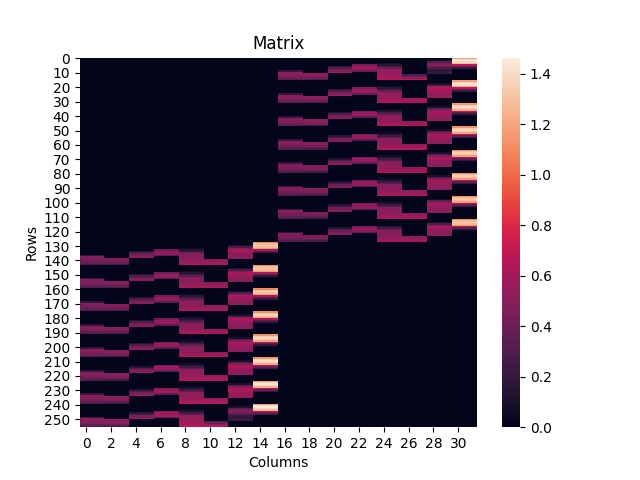
\includegraphics[scale=0.8]{Matrix.png}}
\caption{Исходная матрица системы}
\label{fig:image}
\end{figure}

Видно, что матрица имеет блочную структуру. Для нахождения решения разобьём её на четверти и получим решения для каждой из них. Значения $None$ означают, что решение не удалось получить.

\newpage

\begin{figure}[h]
\center{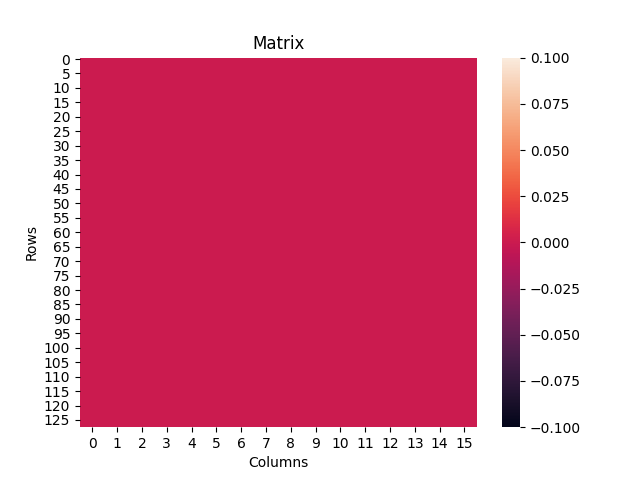
\includegraphics[width=0.5\linewidth]{Quarter_Matrix0.png}}
\caption{Матрица первой четверти}
\label{fig:image}
\end{figure}

Решение для первой четверти:
\begin{equation*}
\begin{pmatrix}
1 : [ None , None ] \\
2 : [ None , None ] \\
3 : [ None , None ] \\
4 : [ None , None ] \\ 
5 : [ None , None ] \\ 
6 : [ None , None ] \\ 
7 : [ None , None ] \\
8 : [ None , None ]
\end{pmatrix}
\end{equation*}

\begin{figure}[h]
\center{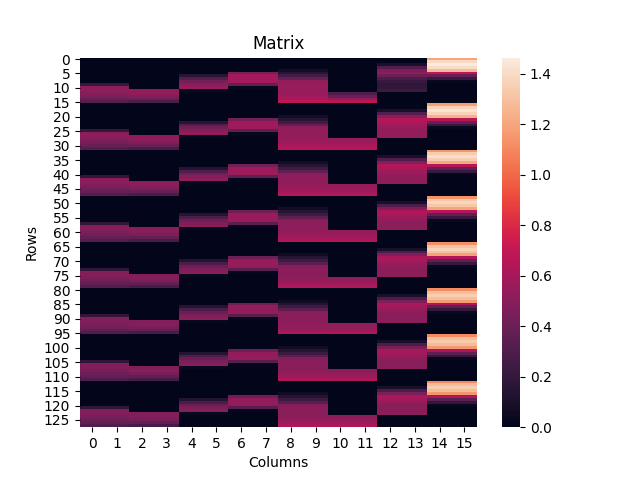
\includegraphics[width=0.5\linewidth]{Quarter_Matrix1.png}}
\caption{Матрица второй четверти}
\label{fig:image}
\end{figure}

Решение для второй четверти:
\begin{equation*}
\begin{pmatrix}
1 : [ 1.000000000000001 , 1.0000000000000004 ] <- \\ 
2 : [ 1.0000000000000013 , 1.0000000000000027 ] -> \\
3 : [ 1.0000000000000548 , 0.9999999999999444 ] <- \\
4 : [ 1.000000000000018 , 0.9999999999999918 ] <- \\ 
5 : [ 1.0000000000000073 , 0.9999999999999802 ] <- \\
6 : [ 1.0000000000000038 , 1.0000000000000044 ] -> \\
7 : [ 1.0000000000000548 , 0.9999999999999444 ] <- \\
8 : [ 1.0 , 1.0 ]    ->
\end{pmatrix}
\end{equation*}
Количество слияний ответов для матрицы второй четверти = 251

\begin{figure}[h]
\center{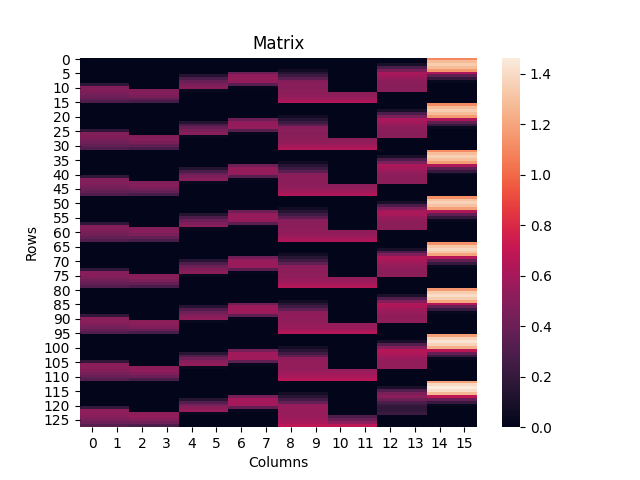
\includegraphics[width=0.5\linewidth]{Quarter_Matrix2.png}}
\caption{Матрица третьей четверти}
\label{fig:image}
\end{figure}

Решение для третьей четверти:
\begin{equation*}
\begin{pmatrix}
1 : [ 1.000000000000001 , 1.0000000000000004 ] <- \\
2 : [ 1.0000000000000013 , 1.0000000000000027 ] -> \\
3 : [ 1.0000000000000548 , 0.999999999999914 ] <- \\ 
4 : [ 1.000000000000018 , 0.9999999999999918 ] <- \\ 
5 : [ 1.0000000000000073 , 0.9999999999999802 ] <- \\ 
6 : [ 1.0000000000000013 , 1.0000000000000044 ] -> \\
7 : [ 1.0000000000000548 , 0.999999999999914 ] <- \\
8 : [ 1.0 , 1.0 ]    ->
\end{pmatrix}
\end{equation*}
Количество слияний ответов для матрицы третьей четверти = 248

\begin{figure}[h]
\center{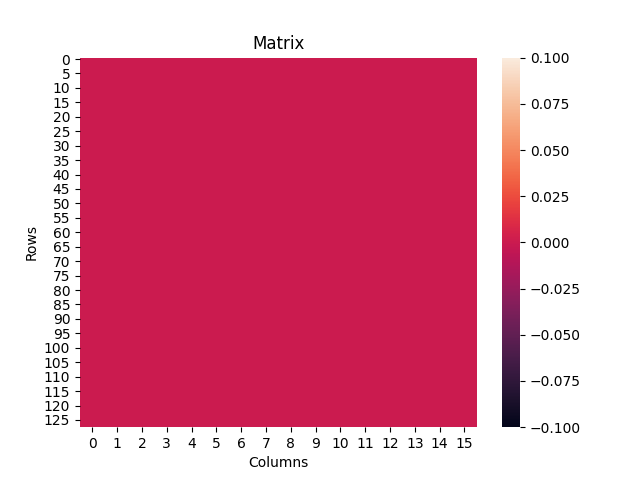
\includegraphics[width=0.5\linewidth]{Quarter_Matrix3.png}}
\caption{Матрица четвертой четверти}
\label{fig:image}
\end{figure}

Решение для четвертой четверти:
\begin{equation*}
\begin{pmatrix}
1 : [ None , None ] \\
2 : [ None , None ] \\
3 : [ None , None ] \\
4 : [ None , None ] \\ 
5 : [ None , None ] \\ 
6 : [ None , None ] \\ 
7 : [ None , None ] \\
8 : [ None , None ]
\end{pmatrix}
\end{equation*}

\newpage
%----------------------------------------------------------------------------------------
%	SECTION 4
%----------------------------------------------------------------------------------------

\section{Литература}
\begin{itemize}
  \item С. П. Шарый, Алгебраический подход во “внешней задаче” для интервальных линейных систем, Фундамент. и прикл. матем., 2002, том 8, выпуск 2, 567–610
  \item А.Н.Баженов, Интервальный анализ. Основы теории, практические применения и учебные примеры.,
  2020, 150-158
  \item Исходный код: \url{https://github.com/ExpressFromSiberia/Interval_Analysis}
  \item Код Никиты Суханова: \url{https://github.com/NikitaSukhanov/Plasma3D}
\end{itemize}

\end{document}
